\chapter{Introduction}\label{Introduction}
Even before computer's invention, inventors have dreamed of creating machine that can think like human. More than 100 years before first programmable computer was actually built, people wondered whether such machines might become intelligent.\\

Today, Artificial Intelligence (AI) is one of the very active area of research with huge amount of practical applications.
We are applying smart and intelligent system everywhere like automating routine tasks, understand speech or images, make diagnoses in medicine and support basic scientific research.

\section{Machine Learning}
 In early days, computers were mainly used for solving problems that are intellectually difficult for human beings but relatively straightforward for computers which can be described by list of formal or mathematical rules. But main challenge is to solve real world tasks that are very easy to perform by human but hard to describe by rule or equation like recognizing spoken words or identifying objects in images.\\

 The difficulties faced by systems relying on hard-coded knowledge suggest that AI systems need the ability to acquire their own knowledge, by extracting patterns from raw data. This capability is known as machine learning. We can formally define machine learning as ``A computer program is said to learn from experience E with respect to some class of tasks T and performance measure P, if its performance at tasks in T, as measured by P, improves with  experience E" .\\

 The introduction of machine learning allowed computers to tackle problems involving knowledge of the real world and make decisions that appear subjective.
 Machine learning is conceptualized as a part of whole  artificial intelligence ecosystem. As you can see in Figure \ref{MLNNDL} a more specialized branch of machine learning is using neural networks as its building blocks.

\begin{figure}[h]
  \centering
  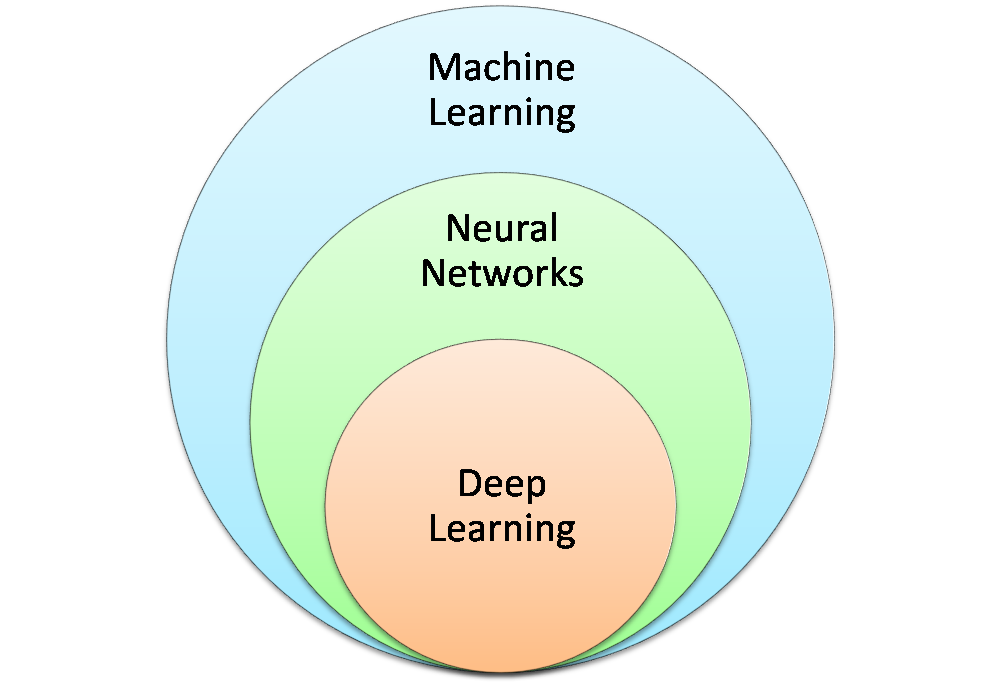
\includegraphics[width=13cm]{img/MLNNDL}
  \caption{Hierarchy of machine learning}\label{MLNNDL}
\end{figure}

 The performance of simple machine learning algorithms depends heavily on the representation of the data they are given. This dependence on representations is a general phenomenon that appears throughout computer science. The choice of representation has an enormous effect on the performance of machine learning algorithms. Once we identify what features to extract, we can teach machine to learn pattern using these features. These tasks can be done using artificial neural networks. By combining multiple neurons we can create artificial neural network which can be trained to perform any given task.\\

As we can see in Figure \ref{learningsteps} process of learning can be divided in two parts:
\begin{tight_enumerate}
  \item Training
  \item Inference
\end{tight_enumerate}

  \begin{figure}[H]
  \centering
  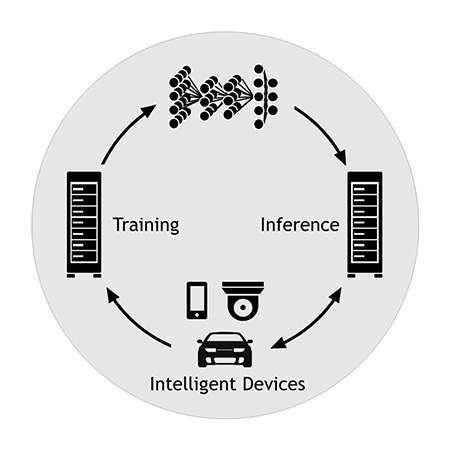
\includegraphics[width=10cm]{img/steps}
  \caption[Steps of learning]{Steps of learning \cite{GTCx}}\label{learningsteps}
\end{figure}

\section{Deep Learning}

Concept of deep learning is nothing new. It was introduced way back in early 80's when computers were not even in day to day usage. First paper on LeNet, a deep convolutional neural network was published in 1989 by Y. LeCun. But back than there was not enough environment available for development of deep neural networks. But recent advancement in field of machine learning started only since 2012 when Alex Krizhevsky successfully demonstrated use of convolutional neural networks by beating traditional methods in ImageNet Large Scale Visual Recognition challenge (ILSVRC) by large margin. This was only possible due to 3 main things \cite{Gettingstartdeeplearninig}:

\begin{itemize}
  \item Use of deep neural network with large number of hidden layer.
  \item Availability of huge amount of data to use for training.
  \item Availability of high performance computing power using GPU.
\end{itemize}

 Ironically, abstract and formal tasks that are among the most difficult mental undertakings for a human being are among the easiest for a computer. From the long time computers have able to defeat the best human chess player, but only recently they are matching some of the abilities of average human beings to recognize objects or speech. A person's everyday life requires an immense amount of knowledge about the world. Much of this knowledge is subjective and intuitive, and therefore difficult to articulate in a formal way. Computers need to capture this same knowledge in order to behave in an intelligent way. One of the key challenges in artificial intelligence is how to get this informal knowledge into a computer.

\section{Benefits of using Deep Learning}
Deep learning is considered as best way to make machine intelligent due to some of following benefits \cite{Gettingstartdeeplearninig}:
\subsection{Robust}
Deep neural networks learn automatically. There is no need to design the features ahead of time. Features are automatically learned to be optimal for specified task.
\subsection{Generalizable}
Same neural network approach can be used in many different applications and different data types for example same network that we use for image labeling can be used for character recognition.
\subsection{Scalable}
Compared to other types of learning performance of deep learning networks improves with more data. These networks are also highly parallelizable due to high number of independent mathematical operations.
